\chapter{Selected Commands of \texttt{thesis} Package}

\section{Quantities and Units}

\begin{table}[!h]
  \caption[An overview of commands]{An overview of commands (use within the mathematical environments).}
  \begin{center}
  	\small
	  \begin{tabular}{|c|c|c|c|}
	    \hline
	    Command    						& Example 					& \LaTeX{} code of example  							& Meaning  \\
	    \hline\hline
	    \verb|\textind{...}|	& $\beta_\textind{max}$ 	& \verb|$\beta_\textind{max}$|	& text-style index \\
	    \hline
	    \verb|\const{...}| 		& $\const{U}_\textind{in}$ 				& \verb|$\const{U}_\textind{in}$|		& constant \\
	    \hline
	    \verb|\var{...}| 		& $\var{u}_\textind{in}$ & \verb|$\var{u}_\textind{in}$| & variable \\
	    \hline
	    \verb|\complex{...}| 	& $\complex{u}_\textind{in}$ & \verb|$\complex{u}_\textind{in}$| & complex variable\\
	    \hline
	    \verb|\vect{...}| 		& $\vect{y}$ 						& \verb|$\vect{y}$| & vector \\
	    \hline
	    \verb|\mat{...}| 	& $\mat{Z}$ 						& \verb|$\mat{Z}$| & matrix \\
	    \hline
	    \verb|\unit{...}| 		& $\unit{kV}$ 						& \verb|$\unit{kV}$|\quad or\ \, \verb|\unit{kV}| & unit \\
	    \hline
	  \end{tabular}
  \end{center}
\end{table}



%\newpage
\section{Symbols}

\begin{itemize}
  \item
    \verb|\E|, \verb|\eul| -- typesets the Euler number: $\eul$,
  \item
    \verb|\J|, \verb|\jmag|, \verb|\I|, \verb|\imag| -- imaginary unit: $\jmag$, $\imag$,
  \item
    \verb|\dif| -- the differential: $\dif$,
  \item
    \verb|\sinc| -- the function $\sinc$,
  \item
    \verb|\mikro| -- typesets the \emph{micro} symbol in roman type%
			\footnote{the symbol comes from package \texttt{textcomp}}: $\mikro$,
	\item
		\verb|\uppi| -- typesets $\uppi$
			(greek pi in roman type, in difference to \verb|\pi|, which typesets~$\pi$).
\end{itemize}
%
All symbols are considered to be used within a~math mode, except \verb|\mikro| that is possible in the text mode as well.
%$\upmikro$


\chapter{Next Appendix}

\begin{figure}[!h]
  \begin{center}
    %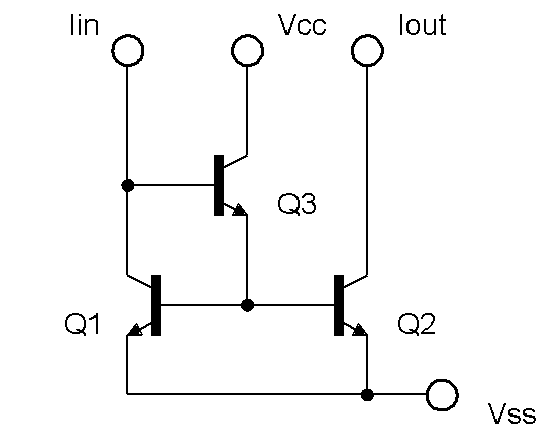
\includegraphics[scale=0.5]{pict/ZlepseneWilsonovoZrcadloNPN}
  \end{center}
  \caption[Wilson mirror]{Improved Wilson current mirror.}
\end{figure}

For inclusion of the vector-based graphics directly via \LaTeX, it is possible to use the \href{https://www.ctan.org/pkg/pgf}{\texttt{TikZ}} package.
Examples of use can be found at the \href{http://www.texample.net/tikz/examples/}{\TeX{}ample} site.
TikZ graphics creation is supported in QTikz and TikzEdt software.




\chapter{Examples of Listing Computer Codes}

\section{Package \texttt{listings}}

Listing computer codes can be handled efficiently via the \href{https://www.ctan.org/pkg/listings}{\texttt{listings}} package.
This package introduces a new environment \texttt{lstlisting} for typesetting computer codes, as for example:
%
\begin{lstlisting}[language={[LaTeX]TeX}]
\section{Package lstlistings}
Listing computer codes can be handled efficiently
via the \texttt{listings} package.
This package introduces a new environment
\texttt{lstlisting} for typesetting computer codes.
\end{lstlisting}
%
The package supports a number of programming languages.
The code to be typeset can be input directly from files on disk.
The package allows row numbering and extracting only selected parts of the code.
The following paragraph is an example of the use of \texttt{listings}:
\bigskip

\noindent
Abbreviations are typeset with the \texttt{acronym} environment:
\label{lst:abbrevs}
\lstinputlisting[language={[LaTeX]TeX}, nolol, numbers=left, firstnumber=6, firstline=6, lastline=6]{text/abbreviation.tex}
%
The width of the input parameter, \verb|HowMuchSpace|, determines the width of the first column.
An example of the definition of abbreviation \acs{symfs} is in Listing~\ref{lst:symfs}.

\shorthandoff{-}
\lstinputlisting%
	[language={[LaTeX]TeX}, frame=single, caption={[Example of code listing]Example of code listing.}, label=lst:symfs, numbers=left, linerange={bsymfvz-\%\%\%\ esymfvz}, includerangemarker=false]{text/abbreviation.tex}
\shorthandon{-}

\noindent
The list is finished with the end of the environment:
\lstinputlisting[language={[LaTeX]TeX}, nolol, numbers=left, firstnumber=26, linerange=26]{text/abbreviation.tex}

\vspace{\fill}

%\noindent
%{\bf Poznámka k~výpisům s~použitím volby jazyka \verb|czech| nebo \verb|slovak|:}\newline
%Pokud Váš zdrojový kód obsahuje znak spojovníku \verb|-|, pak překlad může skončit chybou.
%Ta je způsobená tím, že znak \verb|-| je v~českém nebo slovenském nastavení balíčku \verb|babel| tzv.\ aktivním znakem.
%Přepněte znak \verb|-| na neaktivní příkazem \verb|\shorthandoff{-}| těsně před výpisem a hned za ním jej vraťte na aktivní příkazem \verb|\shorthandon{-}|.
%Podobně jako to je ukázáno ve zdrojovém kódu šablony.


\clearpage

%\section{Listing Matlab code}
Listing \ref{lst:priklad.vypis.kodu.Matlab} contains an example of code for Matlab,
whereas in Listing \ref{lst:priklad.vypis.kodu.C} you find an example in the C~language.

\lstnewenvironment{matlab}[1][]{%
\lstset{language=Matlab,numbers=left,#1}%
}{%
}

\begin{matlab}%
	[frame=single, float=htbp, caption={[Example of the Schur--Cohn test of stability in Matlab]Example of the Schur--Cohn test of stability in Matlab.}, label=lst:priklad.vypis.kodu.Matlab, numberstyle=\scriptsize, numbersep=7pt]
%% Priklad testovani stability filtru

% koeficienty polynomu ve jmenovateli
a = [ 5, 11.2, 5.44, -0.384, -2.3552, -1.2288];
disp( 'Polynom:'); disp(poly2str( a, 'z'))

disp('Kontrola pomoci korenu polynomu:');
zx = roots( a);
if( all( abs( zx) < 1))
    disp('System je stabilni')
else
    disp('System je nestabilni nebo na mezi stability');
end

disp(' '); disp('Kontrola pomoci Schur-Cohn:');
ma = zeros( length(a)-1,length(a));
ma(1,:) = a/a(1);
for( k = 1:length(a)-2)
    aa = ma(k,1:end-k+1);
    bb = fliplr( aa);
    ma(k+1,1:end-k+1) = (aa-aa(end)*bb)/(1-aa(end)^2);
end

if( all( abs( diag( ma.'))))
    disp('System je stabilni')
else
    disp('System je nestabilni nebo na mezi stability');
end
\end{matlab}

\noindent
\begin{minipage}{\linewidth}


%\section{Listing C code}

\begin{lstlisting}%
	[frame=single, numbers=right, caption={[Example of implementation of first canonical form in~C]Example of implementation of first canonical form in~C.}, label=lst:priklad.vypis.kodu.C, basicstyle=\ttfamily\small, keywordstyle=\color{black}\bfseries\underbar]
// first canonical form
short fxdf2t( short coef[][5], short sample)
{
	static int v1[SECTIONS] = {0,0},v2[SECTIONS] = {0,0};
	int x, y, accu;
	short k;

	x = sample;
	for( k = 0; k < SECTIONS; k++){
		accu = v1[k] >> 1;
		y = _sadd( accu, _smpy( coef[k][0], x));
		y = _sshl(y, 1) >> 16;

		accu = v2[k] >> 1;
		accu = _sadd( accu, _smpy( coef[k][1], x));
		accu = _sadd( accu, _smpy( coef[k][2], y));
		v1[k] = _sshl( accu, 1);

		accu = _smpy( coef[k][3], x);
		accu = _sadd( accu, _smpy( coef[k][4], y));
		v2[k] = _sshl( accu, 1);

		x = y;
	}
	return( y);
}
\end{lstlisting}
\end{minipage}







\chapter{Content of the electronic attachment}
An electronic attachment is often a~part of the thesis.
The attachment is uploaded in the BUT information system together with the thesis PDF.
Please use an appropriate file format for the attachment.

It is suggested to comment on every folder, to specify which of the files contains main settings,
to specify which is the main or executable file, what was the setting of the compiler etc.
It is also valuable to specify in which version of the software the code has been tested (e.g.\ Matlab 2018b).
In the case that hardware has been created within the thesis, the electronic attachment must contain all documentation
(for example Eagle files with the printed circuit board layout).

If your attachment contains a~lot of files or folders,
\LaTeX{} package \href{https://www.ctan.org/pkg/dirtree}{\texttt{dirtree}} can become handy,
as in the following example.

\bigskip

{\small
%
\dirtree{%.
.1 /\DTcomment{root of the attached archive}.
.2 logo\DTcomment{logotypes}.
.3 BUT\_abbreviation\_color\_PANTONE\_EN.pdf.
.3 BUT\_color\_PANTONE\_EN.pdf.
.3 FEEC\_abbreviation\_color\_PANTONE\_EN.pdf.
.3 UTKO\_color\_PANTONE\_EN.pdf.
.2 pdf\DTcomment{PDFs (generate them in the information system)}.
.3 assignment-example.pdf.
.3 cover-example.pdf.
.3 titlepage-example.pdf.
.2 text\DTcomment{\LaTeX{} source codes of the text}.
.3 abbreviation.tex.
.3 appendix.tex.
.3 bibliography.tex.
.3 conclusion.tex.
.3 introduction.tex.
.3 results.tex.
.3 solution.tex.
.2 template-thesis.tex\DTcomment{main file of the thesis}.
.2 template-presentation.tex\DTcomment{main file of the slides for presentation}.
.2 thesis.sty\DTcomment{package for typesetting final theses at BUT}.
}
}
